\begin{question}
  \hspace*{\fill} [Note Maximale: 16]\par
  \medskip
  \noindent Considérez le cercle suivant de centre $O$ et de rayon $r$.\par
  \medskip
  \begin{center} % or flushleft or flushright
    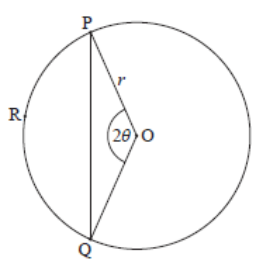
\includegraphics[scale=0.4]{figure_x6}\par
    \noindent Les points $P$, $R$ et $Q$ sont sur la circonférence, $\angle\,POQ = 2\theta$, pour $0 \le \theta \le \frac{\pi}{2}$.\par
  \end{center} % or flushleft or flushright

  \begin{enumerate}[label=(\alph*)]
    \item Utilisez la loi des cosinus pour montrer que $PQ = 2r\,sin\,\theta$.\hspace*{\fill} [4]
    \item Soit $l$ la longueur de larc $PRQ$.\par
      Étant donnez que $1,3PQ - l = 0$, trouvez la valeur de $\theta$.\hspace*{\fill} [5]
    \item Considérez la fonction $f(\theta) = 2,6\,sin\,\theta - 2\theta$, pour $0 \le \theta \frac{\pi}{2}$.
      \begin{enumerate}[label=(\roman*)]
        \item Esquissez la représentation graphique de $f$.
        \item Donnez la racine de $f(\theta) = 0$.\hspace*{\fill} [4]
      \end{enumerate}
    \item Utilisez la courbe $f$ pour trouver les valeurs de $\theta$ pour lesquelles $l < 1,3\,PQ$.\hspace*{\fill} [3]
  \end{enumerate}
\end{question}
